% DO NOT COMPILE THIS FILE DIRECTLY!
% This is included by the the driver file (FlipBeamerTemplate.tex).

{ %% This is a total kludge for a fancy title page background
%\setbeamertemplate{sidebar right}{\llap{\includegraphics[width=\paperwidth,height=\paperheight]{BG_upper}}}
\begin{frame}[c]%{\phantom{title page}} 
% The \phantom{title page} is a kludge to get the red bar on top
 \titlepage
\end{frame}
}

\begin{frame}
\frametitle{\textit{Background}}
Let 
\[
Y = \left(y_1,\dots, y_p\right)', \quad \left(t_1,\dots, t_p\right)'
\]
denote the random vector of observations and their associated measurement times, where 
\begin{align*}
 Cov\left(Y\right) = \Sigma = \left[ \sigma_{ij} \right] 
\end{align*}

\begin{itemize}
\item \nt{Dimensionality: the number of parameters is quadratic in $p$.} \pause
\item \nt{Covariance estimates should satisfy the positive definite constraint:}
\begin{equation*}
 		c'\Sigma c = \sum_{i,j = 1}^p c_i c_j \sigma_{ij} \ge 0
\end{equation*} \pause
\item \nt{Observation times may be irregular or subject-specific.} 
\end{itemize}
\end{frame}



%\begin{frame}
%\frametitle{}
%\begin{equation*} \label{eq:sample-covariance-matrix}
%S = \frac{1}{N-1} \sum_{i = 1}^N \left(Y_i - \bar{Y}\right)\left(Y_i - \bar{Y}\right)', \;\;\bar{Y} = \frac{1}{N} \sum_{i=1}^N Y_i
%\end{equation*}
%\noindent
%
%\begin{center}
%
%\begin{tikzpicture}
%\node[draw,fill=ash,
%align= center,
%text=white,text width=2cm, 
%      minimum width=2cm,
%    minimum height=1cm] (1) at (0,2) {Parametric Models} ;
%\node[draw,fill=ash,
%align= center,
%text=white,text width=2cm, 
%      minimum width=2cm,
%    minimum height=1cm] (2) at (7,2) {$S$};
%\node[draw,fill=ash,text=white,text width=3cm, 
%      minimum width=2cm,
%      align= center,
%    minimum height=1cm] (3) at (0,0) {high bias, low variance};
%\node[draw,fill=ash,text=white,text width=3cm, 
%      minimum width=2cm,
%      align= center,
%    minimum height=1cm] (4) at (7,0){low bias, high variance} ;
%\draw[-,draw=hilight] (1) to (2);
%\draw[-,draw=hilight] (1) to (3);
%\draw[-,draw=hilight] (2) to (4);
%  \end{tikzpicture}
%\end{center}
%\end{frame}



\begin{frame}
\frametitle{\textit{Outline}}

\begin{itemize}
\item \nt{Background: A Review of Covariance Estimation for Longitudinal Data}
	\begin{itemize}
	\item \nt{The Cholesky Decomposition}
	\end{itemize}
\item \nt{A Reproducing Kernel Hilbert Space Framework for Covariance Estimation}
\item \nt{Tensor Product P-splines for Covariance Estimation}
\item \nt{Simulation Studies}
\item \nt{Data Analysis: Cattle Weights}
\end{itemize}
\end{frame}



\begin{frame}{\textit{Common approaches to covariance estimation}}

\centering

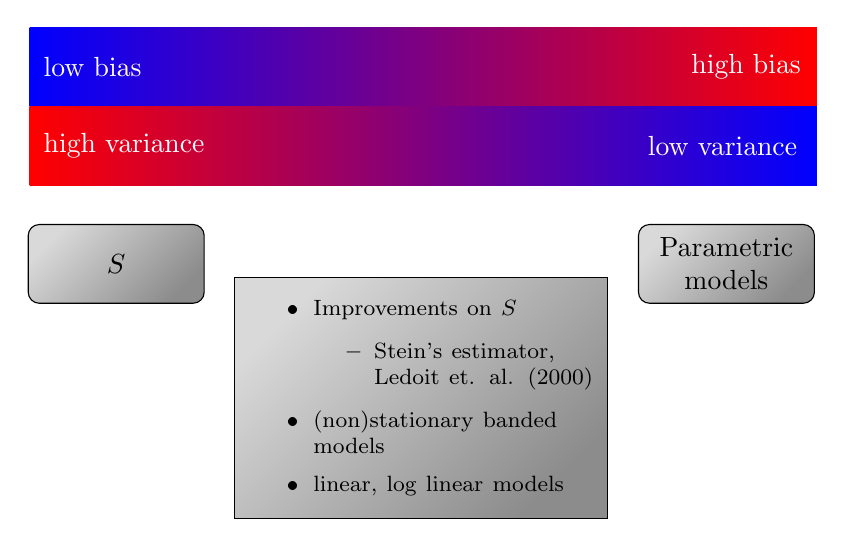
\begin{tikzpicture} 
\draw[-,draw=white, thick] (1.1,2.8) to (8.85,2.8);
\draw[-,draw=white, thick] (8.85,2.2) to (8.85,2.8);
\draw[-,draw=white, thick] (1.1,2.2) to (1.1,2.8);
\draw[-,draw=white, thick] (4.975,2.425) to (4.975,2.8);
\node [draw, top color=gray!30!, bottom color=gray!90, shading angle=45, text width=2cm, 
text centered, rounded corners, minimum height=10mm] (s) at (1.1,2) {$S$};
\node [draw, top color=gray!30!, bottom color=gray!90, shading angle=45, text width=2cm, 
text centered, rounded corners, minimum height=10mm] (s) at (8.85,2) {Parametric models};
\shade[left color=blue,right color=red] (0,4) rectangle (10,5);
\shade[left color=red,right color=blue] (0,4) rectangle (10,3);
\node[align = right, text=white]  at (9.1,4.5) {high bias} ;
\node[text=white,align=left]  at (.8,4.5) {low bias} ;
\node[text=white,align=right]  at (8.8,3.5) {low variance} ;
\node[text=white,align=left]  at (1.2,3.5) {high variance} ;
\node [draw,text width=4.5cm, minimum height=20mm,top color=gray!30!,
bottom color=gray!90, shading angle=45,] at (4.975,0.3) {\vbox {\footnotesize
    {\begin{itemize}
        \item Improvements on $S$ 
         \begin{itemize}
        \item Stein's estimator, Ledoit et. al. (2000)
        \end{itemize}
        \item (non)stationary banded models
        \item linear, log linear models
    \end{itemize}}
}};

\end{tikzpicture}


\end{frame}

%%%%%%%%%%%%%%%%%%%%%%%%%%%%%%%%%%%%%%%%%%%%%%%%%%%%%%%%%%%%%%%%%%%%%%%%%%%%
%%%%%%%%%%%%%%%%%%%%%%%%%%%%%%%%%%%%%%%%%%%%%%%%%%%%%%%%%%%%%%%%%%%%%%%%%%%%
%%%%%%%%%%%%%%%%%%%%%%%%%%%%%%%%%%%%%%%%%%%%%%%%%%%%%%%%%%%%%%%%%%%%%%%%%%%%
%%%%%%%%%%%%%%%%%%%%%%%%%%%%%%%%%%%%%%%%%%%%%%%%%%%%%%%%%%%%%%%%%%%%%%%%%%%%



%%%%%%%%%%%%%%%%%%%%%%%%%%%%%%%%%%%%%%%%%%%%%%%%%%%%%%%%%%%%%%%%%%%%%%%%%%%%
%%%%%%%%%%%%%%%%%%%%%%%%%%%%%%%%%%%%%%%%%%%%%%%%%%%%%%%%%%%%%%%%%%%%%%%%%%%%


%
%\begin{frame}
%\frametitle{\emph{Matrix Decompositions}}
%
%	\begin{columns}[T]
%	
%	\begin{column}{0.5\textwidth}
%	\footnotesize
%	\textbf{The Variance-Correlation Decomposition} 
%	\begin{align*}%\label{eq:variance-correlation-decomposition}
%	\Sigma &= DRD,\\
%	 D &= \mbox{diag}\left(\sqrt{\sigma_{11}},\dots , \sqrt{\sigma_{pp}}\right), \quad R = \left[ \rho_{ij} \right]
%	\end{align*}
%	\begin{itemize}
%	\item standard deviations are on the same scale as the responses,
%	\item $R$, $D$ can be estimated separately 
%	\item $R$ is constrained; typically modeled with parsimonious, structured correlation matrices
%	\end{itemize}
%
%	\end{column}
%	
%	\begin{column}{0.55\textwidth}
%	\footnotesize
%	\textbf{The Spectral Decomposition:} 
%	\begin{equation*}% \label{eq:spectral-decomposition}
%	\Sigma = P \Lambda P' = \sum_{i = 1}^p \lambda_i e_i e'_i,
%	\end{equation*}	\footnotesize
%	\begin{itemize}
%	\item $e_i$, $\lambda_i$ are the coefficients and variances of the $p$ principal components.
%	\item $P$ constrained by orthogonality.
%	\end{itemize}
%	\textbf{The Matrix Logarithm:} 
%	\begin{align*}% \label{eq:spectral-decomposition}
%	\log \Sigma &= P \left(\log\Lambda\right) P' \\
%	&= \sum_{i = 1}^p \log\left(\lambda_i \right)e_i e'_i,
%	\end{align*}	\footnotesize
%	\begin{itemize}
%	\item Unconstrained, but the $\log \lambda_i$ lack any statistical interpretation.
%	\end{itemize}
%	\end{column}
%	\end{columns}
%	
%
%\end{frame}
%





\begin{frame}
\frametitle{\emph{The Modified Cholesky decomposition}}
For any positive definite $\Sigma$, there exists a unique lower-triangular matrix $C =  \left[c_{ij} \right]$, $c_{ii}> 0$:

\begin{equation*}
\Sigma = CC',
\end{equation*}

Let $D^{1/2} = diag\left( c_{11},\dots, c_{pp} \right)$, $L = D^{-1/2}C$, then 

\begin{equation*}
\Sigma =L D L'. %= CD^{-1/2}DD^{-1/2}C' = 
\end{equation*}

The \nt{\textbf{modified Cholesky decomposition} (MCD)} of $\Sigma$ is given by
\nt{\begin{equation}\label{eq:modified-cholesky-decomposition}
D = T\Sigma T',
\end{equation}}
where {$T = L^{-1}$}. The lower triangular entries of $T$ are \textit{unconstrained}.

\end{frame}





\begin{frame}
\frametitle{\emph{Statistical Interpretation of $\left(T,D\right)$}}{}
\footnotesize
Let $\hat{y}_t$ be the linear least-squares predictor of $y_t$ based on previous measurements $y_{t-1}, \dots , y_1$ and $\epsilon_t = y_t - \hat{y}_t$ denote the corresponding mean zero prediction error with variance $Var\left(\epsilon_t\right) = \sigma_t^2$. We can find unique scalars $\phi_{tj}$:

\nt{\begin{equation*} \label{eq:mcd-ar-model}
y_t = \left\{ \begin{array}{ll} \epsilon_t, & t = 1\\
\sum_{j = 1}^{t-1} \phi_{tj} y_j + \epsilon_t, & t = 2, \dots, p,
\end{array}\right.
\end{equation*}}

where $D = Cov\left( \epsilon \right) = diag\left( \sigma_1^2,\dots,\sigma_p^2, \right)$. Then

\begin{align*}
\underbrace{\begin{bmatrix}
\epsilon_1 \\
\epsilon_2 \\ \vdots \\\epsilon_{p-1} \\ \epsilon_p
\end{bmatrix}}_{\nt{\epsilon}} = \underbrace{\begin{bmatrix}
1&&&&\\
-\phi_{21}&1&&&\\
-\phi_{31}&-\phi_{32}&1&&\\
\vdots &&&\ddots& \\
-\phi_{p1}&-\phi_{p2}& \dots & -\phi_{p,p-1}&1\\
\end{bmatrix}}_{\nt{T}}
\underbrace{\begin{bmatrix}
y_1 \\
y_2 \\ \vdots \\ y_{p-1}\\y_p
\end{bmatrix}}_{\nt{Y}}
\end{align*}

Taking the covariance on both sides gives the \nt{MCD \eqref{eq:modified-cholesky-decomposition}}.
\end{frame}


\begin{frame}{\textit{The coefficients and prediction error variances of successive regressions are unconstrained.}}{}
\begin{columns}[T]
\begin{column}{0.5\textwidth}
The \textbf{generalized autoregressive parameters} $\phi_{tj}$ and \textbf{log innovation variances} $\log \sigma_j^2$ are unconstrained but  
\[
\hat{\Sigma}^{-1} = \hat{T}' \hat{D}^{-1} {T}
\]
is guaranteed to be positive definite.
\end{column}
\begin{column}{0.5\textwidth}
\footnotesize
\begin{tabular}{cccccc}
 $y_{1}$&$y_{2}$ & $y_{3}$ & $\dots$ &$y_{p-1}$& $y_{p}$\\ \hline
 $1$& &&&&\\
$\phi_{21}$& $1$ &&&& \\
$\phi_{31}$& $\phi_{32}$& $1$ &&& \\ 
$\vdots$ & $\vdots$ & & $\ddots$&& \\
$\vdots$ & $\vdots$ & && $\ddots$& \\
$\phi_{p1}$& $\phi_{p2}$&$\dots$ &$\dots$ &$\phi_{p,p-1}$ & $1$\\ \hline
$\sigma_1^2$ & $\sigma_2^2$ & $\dots$&$\dots$ &$\sigma_{p-1}^2$ &$\sigma_p^2$
\end{tabular} 
\end{column}
\end{columns}

\end{frame}



\begin{frame}{\textit{The ideal form of longitudinal data:}}

\centering
\begin{tabular}{cc|cccccc}
\multicolumn{8}{c}{Time}\\
& & $1$&$2$ &  $\dots$ & $t$ & $\dots$ & $p$ \\ \hline
& 1 & $y_{11}$&$y_{12}$ &$\dots$ & $y_{1t}$ & $\dots$& $y_{1p}$ \\
& 2 & $y_{21}$&$y_{22}$ &$\dots$ & $y_{2t}$ & $\dots$& $y_{2p}$ \\
\begin{rotate}{90}%
\mbox{Unit}\end{rotate} & $\vdots$ &$\vdots$&$\vdots$ & &$\vdots$ & & $\vdots$ \\
& $i$ & $y_{i1}$&$y_{i2}$ &$\dots$ & $y_{it}$ & $\dots$& $y_{ip}$ \\
 & $\vdots$ &$\vdots$&$\vdots$ & &$\vdots$ & & $\vdots$ \\
 & $N$ & $y_{N1}$&$y_{N2}$ &$\dots$ & $y_{Nt}$ & $\dots$& $y_{Np}$ \\
\end{tabular}
\end{frame}






\begin{frame}{\emph{Maximum Normal Likelihood Estimation for the Cholesky Decomposition}}{The MLE for $\left(T,D\right)$ has closed form under the Gaussian likelihood.}

For  $Y_1,\dots , Y_N \sim N\left(0_p, \Sigma\right)$ and $S = N^{-1}\sum_{i=1}^N Y_iY'_i$,

\begin{align}
\begin{split} \label{eq:regular-cholesky-log-likelihood}
-2\ell\left(\Sigma \vert Y_1,\dots, Y_N\right) &= \sum_{i = 1}^N \left( \log \vert \Sigma \vert  + Y'_i \Sigma^{-1}Y_i\right) \\
& = N \log \vert D \vert + N \mbox{tr}\left(D^{-1}TST'\right)
\end{split}
\end{align}
\noindent
is quadratic in $T$ for fixed $D$, so the MLE for the $\phi_{tj}$ has closed form. Similarly, the MLE for $D$ for fixed $T$ has closed form. 
\end{frame}






\begin{frame}{\emph{Parametric Models for the Cholesky Decomposition}}{} \label{polynomial-mcd-model}

Pourahmadi (2000), Pan andMackenzie (2003) suggest modeling $\phi_{tj}$, $\sigma^2_{t}$ with covariates, letting 

\begin{align*}
\begin{split}  \label{eq:GARP-IV-parametric-model}
\phi_{jk} &= x'_{jk} \gamma \\
\log \sigma^2_{j} &= z'_{j}\lambda. 
\end{split}
\end{align*}

Common choices for the covariates $x_{jk}$ and $z_j$ are

\begin{align*}
x'_{jk} &= \left(1, t_j - t_k, \left(t_j - t_k\right)^2,\dots, \left(t_j - t_k\right)^{d-1}\right)', \\
z'_{j}  &= \left(1, t_j, \dots, t_j^{q-1}\right)'.
\end{align*} \label{eq:mcd-polynomial-model}
\noindent
Polynomial orders $d$ and $q$ are tuning parameters chosen by a model selection criterion (BIC, AIC).
\vspace{1cm}

\hyperlink{simulation-studies-benchmark-estimators}{\beamerskipbutton{Simulations}}

\end{frame}


%\begin{frame}{Other Models for the Cholesky Decomposition}{}
%\footnotesize
%
%\begin{itemize}
%\item \cite{wu2003nonparametric,huang2006covariance,dahlhaus1997fitting} extend model~\eqref{eq:mcd-ar-model} with univariate varying coefficient models:
%	\begin{equation} \label{eq:one-dimensional-mcd-vc-model}
%	y_t = \sum_{j = 1}^{t-1} f_{j}\left( t \right) y_{t-j} + \sigma^2\left(t\right)
%	\end{equation}
%	%\cite{wu2003nonparametric} give details of smoothing and selection of the order $k$ of the autoregression under the assumption that the $N$ subjects share common observation times.
%\item \cite{smith2002parsimonious} propose parsimonious model for $\Sigma$ using a prior distribution that allows for zero entries in $T$  
%\item \cite{huang2006covariance} use $L_1$-penalized likelihood to estimate $T$ for Gaussian data. 
%\item \cite{levina2008sparse} use penalized maximum likelihood with a `nested Lasso' penalty imposing an adaptive bandwidth for each row of $T$ with balanced data.
%\end{itemize}
%\end{frame}


%\begin{frame}{Accommodating Unbalanced Data}{by treating $\phi$ as a continuous bivariate function.}
%
%  \begin{tikzpicture}
%    \node (yend) at (-0.35, 5.5)  {};
%    \node (xend) at ( 5.5, -0.35)  {};
%    \node at (0,6) {$1$};
%    \node at (1,5) {$1$};
%    \node at (2,4) {$1$};
%    \node at (3,3) {$1$};
%    \node at (4,2) {$1$};
%    \node at (5,1) {$1$};
%    \node at (6,0) {$1$};
%%    \path[top color=gray, bottom color=gray!60] (-0.35,-0.35) -- (-0.35,5.85)  -- (5.85,-0.35) --  (-0.35,-0.35);
%    \node at (0,5) {$\phi_{21}$};
%   \node at (0,4) {$\phi_{31}$};
% \node at (0,3) {$\phi_{41}$};
% \fill [white] (0,0.7) circle [radius=1pt];
% \fill [white] (0,1) circle [radius=1pt]; 
%  \fill [white] (0,1.3) circle [radius=1pt]; 
%  \node at (1,3) {$\phi_{42}$};
%   \node at (2,3) {$\phi_{43}$};
% \node at (0,2) {$\phi_{51}$};
%  \node at (1,2) {$\phi_{52}$};
%      \node at (3,2) {$\phi_{54}$};
%%\fill [mint] (2,2) circle [radius=2pt];
%   \node at (0,0) {$\phi_{p1}$};
%   \node at (1,0) {$\phi_{p2}$};
%      \node at (2,0) {$\phi_{p3}$};
%   \node at (5,0) {$\phi_{p, p-1}$};
%    \fill [white] (3,0) circle [radius=1pt];
% \fill [white] (3.5,0) circle [radius=1pt]; 
%  \fill [white] (4,0) circle [radius=1pt]; 
%   \node at (1,4) {$\phi_{32}$};
%%  \path[->, color=mint, line width=1] (2,2) edge [out = 50,in = 160] (6,5);
%% \node at (7.5,5) {\textcolor{mint}{$\phi_{54} = \phi\left(t_5,t_4\right)$}};
%   \end{tikzpicture} \\
%\end{frame}





\begin{frame}{Accommodating Unbalanced Data}{Subjects 1 and 2 have different measurement times.}

  \begin{tikzpicture}
    \node (yend) at (-0.35, 5.5)  {};
    \node (xend) at ( 5.5, -0.35)  {};
    \node at (0,6) {$1$};
    \node at (1,5) {$1$};
    \node at (2,4) {$1$};
    \node at (3,3) {$1$};
    \node at (4,2) {$1$};
    \node at (5,1) {$\ddots$};
    \node at (6,0) {$1$};
     \node at (0,6) {$1$};
    \node at (5,5.5) {\textcolor{paleale}{$t_1 = \left( t_{11}, t_{12}, \dots, t_{1p_1} \right)'$}};
     \node at (5,5) {\textcolor{pink}{$t_2 = \left( t_{21}, t_{22}, \dots, t_{2p_2} \right)'$}};
    \path[top color=gray, bottom color=gray!60] (-0.35,-0.35) -- (-0.35,5.85)  -- (5.85,-0.35) --  (-0.35,-0.35);
 \fill [white] (0,0.7) circle [radius=1pt];
 \fill [white] (0,1) circle [radius=1pt]; 
  \fill [white] (0,1.3) circle [radius=1pt]; 
  \node at (2,1) {\textcolor{mint}{$\left( t_{ij}, t_{ik}\right):\; t_{ij} > t_{ik}$}};
 \node at (4,2) {$1$};
  \node at (4,2) {$1$};

    \fill[white] (2.9,0) circle [radius=1pt];
  \fill[white] (3.5,0) circle [radius=1pt]; 
  \fill[white] (4.1,0) circle [radius=1pt]; 
  
  \fill[paleale]  (0,4.8) circle [radius=2.5pt];
    \fill [paleale]  (0,4) circle [radius=2.5pt];
 \fill [paleale]  (0,2.5) circle [radius=2.5pt];
   \fill[paleale]  (1.2,2.5) circle [radius=2.5pt];
       \fill[paleale]  (2,2.5) circle [radius=2.5pt];
  \fill[paleale] (0,2) circle [radius=2.5pt];
   \fill[paleale] (1,2) circle [radius=2.5pt];
       \fill[paleale] (2.5,2) circle [radius=2.5pt];
    \fill[paleale] (0,0)  circle [radius=2.5pt];
    \fill[paleale] (1.2,0)  circle [radius=2.5pt];
       \fill[paleale] (2,0) circle [radius=2.5pt];
    \fill[paleale] (5,0) circle [radius=2.5pt];
    \fill[paleale] (1.2,4) circle [radius=2.5pt];
      \fill[paleale]  (0,4.8) circle [radius=2.5pt];     

 \fill [pink]  (0.2,5) circle [radius=2.5pt];
  \fill [pink]  (0.2,4) circle [radius=2.5pt];
 \fill [pink]  (0.2,3) circle [radius=2.5pt];
   \fill[pink] (0.2,2.3) circle [radius=2.5pt];
       \fill[pink] (0.2,0.3)  circle [radius=2.5pt];
           \fill[pink] (1,0.3)  circle [radius=2.5pt];
   \fill[pink]  (1,2.3) circle [radius=2.5pt];
    \fill[pink] (1,3) circle [radius=2.5pt];
    \fill[pink] (1,4) circle [radius=2.5pt];
%   \fill[pink] (2, 1) circle [radius=2.5pt];
  \fill[pink] (2,0.3) circle [radius=2.5pt];
  \fill[pink] (2.7,2.3) circle [radius=2.5pt];
    \fill[pink] (5,.3) circle [radius=2.5pt];
\draw[<-, color = mint] (-0.55,-0.55) -- (-0.55,5.85); 
\draw[->, color = mint] (-0.55,-0.65) -- (5.95,-0.65); 
% \node at (0,5) {$\phi_{21}$};
%   \node at (0,4) {$\phi_{31}$};
% \node at (0,3) {$\phi_{41}$};
%  \node at (1,3) {$\phi_{42}$};
%   \node at (2,3) {$\phi_{43}$};
% \node at (0,2) {$\phi_{51}$};
%  \node at (1,2) {$\phi_{52}$};
%      \node at (3,2) {$\phi_{54}$};
%   \node at (0,0) {$\phi_{p1}$};
%   \node at (1,0) {$\phi_{p2}$};
%      \node at (2,0) {$\phi_{p3}$};
%   \node at (5,0) {$\phi_{p, p-1}$};
%      \node at (1,4) {$\phi_{32}$};
%        \node at (2,2) {$\phi_{53}$};
%    \node at (2,0) {$\phi_{p3}$};
%   \node at (5,0) {$\phi_{p, p-1}$};
 \node at (-0.75,2.5) {\textcolor{mint}{$t$}};
  \node at (2.5,-0.85) {\textcolor{mint}{$s$}};
   \end{tikzpicture} \\
\end{frame}





\begin{frame}{Accommodating Unbalanced Data}{Subjects 1 and 2 have different measurement times.}

  \begin{tikzpicture}
    \node (yend) at (-0.35, 5.5)  {};
    \node (xend) at ( 5.5, -0.35)  {};
    \node at (0,6) {$1$};
    \node at (1,5) {$1$};
    \node at (2,4) {$1$};
    \node at (3,3) {$1$};
    \node at (4,2) {$1$};
    \node at (5,1) {$\ddots$};
    \node at (6,0) {$1$};
    \path[top color=gray, bottom color=gray!60] (-0.35,-0.35) -- (-0.35,5.85)  -- (5.85,-0.35) --  (-0.35,-0.35);
 \fill [white] (0,0.7) circle [radius=1pt];
 \fill [white] (0,1) circle [radius=1pt]; 
  \fill [white] (0,1.3) circle [radius=1pt]; 

    \fill[white] (2.9,0) circle [radius=1pt];
  \fill[white] (3.5,0) circle [radius=1pt]; 
  \fill[white] (4.1,0) circle [radius=1pt]; 
  
  \fill[paleale]  (0,4.8) circle [radius=2.5pt];
    \fill [paleale]  (0,4) circle [radius=2.5pt];
 \fill [paleale]  (0,2.5) circle [radius=2.5pt];
   \fill[paleale]  (1.2,2.5) circle [radius=2.5pt];
       \fill[paleale]  (2,2.5) circle [radius=2.5pt];
  \fill[paleale] (0,2) circle [radius=2.5pt];
   \fill[paleale] (1,2) circle [radius=2.5pt];
       \fill[paleale] (2.5,2) circle [radius=2.5pt];
    \fill[paleale] (0,0)  circle [radius=2.5pt];
    \fill[paleale] (1.2,0)  circle [radius=2.5pt];
       \fill[paleale] (2,0) circle [radius=2.5pt];
    \fill[paleale] (5,0) circle [radius=2.5pt];
    \fill[paleale] (1.2,4) circle [radius=2.5pt];
      \fill[paleale]  (0,4.8) circle [radius=2.5pt];     

 \fill [pink]  (0.2,5) circle [radius=2.5pt];
  \fill [pink]  (0.2,4) circle [radius=2.5pt];
 \fill [pink]  (0.2,3) circle [radius=2.5pt];
   \fill[pink] (0.2,2.3) circle [radius=2.5pt];
       \fill[pink] (0.2,0.3)  circle [radius=2.5pt];
           \fill[pink] (1,0.3)  circle [radius=2.5pt];
   \fill[pink]  (1,2.3) circle [radius=2.5pt];
    \fill[pink] (1,3) circle [radius=2.5pt];
    \fill[pink] (1,4) circle [radius=2.5pt];
%   \fill[pink] (2, 1) circle [radius=2.5pt];
  \fill[pink] (2,0.3) circle [radius=2.5pt];
  \fill[pink] (2.7,2.3) circle [radius=2.5pt];
    \fill[pink] (5,.3) circle [radius=2.5pt];

 \node at (0,5) {$\phi_{21}$};
   \node at (0,4) {$\phi_{31}$};
 \node at (0,3) {$\phi_{41}$};
  \node at (1,3) {$\phi_{42}$};
   \node at (2,3) {$\phi_{43}$};
 \node at (0,2) {$\phi_{51}$};
  \node at (1,2) {$\phi_{52}$};
      \node at (3,2) {$\phi_{54}$};
   \node at (0,0) {$\phi_{p1}$};
   \node at (1,0) {$\phi_{p2}$};
      \node at (2,0) {$\phi_{p3}$};
   \node at (5,0) {$\phi_{p, p-1}$};
      \node at (1,4) {$\phi_{32}$};
        \node at (2,2) {$\phi_{53}$};
    \node at (2,0) {$\phi_{p3}$};
   \node at (5,0) {$\phi_{p, p-1}$};
    \node at (-0.75,2.5) {\textcolor{mint}{$t$}};
  \node at (2.5,-0.85) {\textcolor{mint}{$s$}};
   \draw[<-, color = mint] (-0.55,-0.55) -- (-0.55,5.85); 
\draw[->, color = mint] (-0.55,-0.65) -- (5.95,-0.65); 
   \end{tikzpicture} \\
\end{frame}



\begin{frame}{Accommodating Unbalanced Data}{by treating $\phi$ as a continuous bivariate function.}

  \begin{tikzpicture}
    \node (yend) at (-0.35, 5.5)  {};
    \node (xend) at ( 5.5, -0.35)  {};
    \node at (0,6) {$1$};
    \node at (1,5) {$1$};
    \node at (2,4) {$1$};
    \node at (3,3) {$1$};
    \node at (4,2) {$1$};
    \node at (5,1) {$\ddots$};
    \node at (6,0) {$1$};
    \path[top color=gray, bottom color=gray!60] (-0.35,-0.35) -- (-0.35,5.85)  -- (5.85,-0.35) --  (-0.35,-0.35);
    \node at (0,5) {$\phi_{21}$};
   \node at (0,4) {$\phi_{31}$};
 \node at (0,3) {$\phi_{41}$};
 \fill [white] (0,0.7) circle [radius=1pt];
 \fill [white] (0,1) circle [radius=1pt]; 
  \fill [white] (0,1.3) circle [radius=1pt]; 
  \node at (1,3) {$\phi_{42}$};
   \node at (2,3) {$\phi_{43}$};
 \node at (0,2) {$\phi_{51}$};
  \node at (1,2) {$\phi_{52}$};
      \node at (3,2) {$\phi_{54}$};
   \node at (0,0) {$\phi_{p1}$};
   \node at (1,0) {$\phi_{p2}$};
      \node at (2,0) {$\phi_{p3}$};
   \node at (5,0) {$\phi_{p, p-1}$};
    \fill [white] (2.9,0) circle [radius=1pt];
 \fill [white] (3.5,0) circle [radius=1pt]; 
  \fill [white] (4.1,0) circle [radius=1pt]; 
   \node at (1,4) {$\phi_{32}$};
\draw[<-, color = mint] (-0.55,-0.55) -- (-0.55,5.85); 
\draw[->, color = mint] (-0.55,-0.65) -- (5.95,-0.65); 
 \node at (-0.75,2.5) {\textcolor{mint}{$t$}};
  \node at (2.5,-0.85) {\textcolor{mint}{$s$}};
       \node at (2,0) {$\phi_{p3}$};
   \node at (5,0) {$\phi_{p, p-1}$};
%   \fill [mint] (2,2) circle [radius=2pt];
%    \path[->, color=mint, line width=1] (2,2) edge [out = 50,in = 160] (6,5);
% \node at (7.5,5) {\textcolor{mint}{$\phi_{54} = \phi\left(t_5,t_4\right)$}};
   \end{tikzpicture} \\
\end{frame}


\begin{frame}{Accommodating Unbalanced Data}{by treating $\phi$ as a continuous bivariate function.}

  \begin{tikzpicture}
    \node (yend) at (-0.35, 5.5)  {};
    \node (xend) at ( 5.5, -0.35)  {};
    \node at (0,6) {$1$};
    \node at (1,5) {$1$};
    \node at (2,4) {$1$};
    \node at (3,3) {$1$};
    \node at (4,2) {$1$};
    \node at (5,1) {$\ddots$};
    \node at (6,0) {$1$};
    \path[top color=gray, bottom color=gray!60] (-0.35,-0.35) -- (-0.35,5.85)  -- (5.85,-0.35) --  (-0.35,-0.35);
    \node at (0,5) {$\phi_{21}$};
   \node at (0,4) {$\phi_{31}$};
 \node at (0,3) {$\phi_{41}$};
 \fill [white] (0,0.7) circle [radius=1pt];
 \fill [white] (0,1) circle [radius=1pt]; 
  \fill [white] (0,1.3) circle [radius=1pt]; 
  \node at (1,3) {$\phi_{42}$};
   \node at (2,3) {$\phi_{43}$};
 \node at (0,2) {$\phi_{51}$};
  \node at (1,2) {$\phi_{52}$};
      \node at (3,2) {$\phi_{54}$};
   \node at (0,0) {$\phi_{p1}$};
   \node at (1,0) {$\phi_{p2}$};
      \node at (2,0) {$\phi_{p3}$};
   \node at (5,0) {$\phi_{p, p-1}$};
    \fill [white] (2.9,0) circle [radius=1pt];
 \fill [white] (3.5,0) circle [radius=1pt]; 
  \fill [white] (4.1,0) circle [radius=1pt]; 
   \node at (1,4) {$\phi_{32}$};
\draw[<-, color = mint] (-0.55,-0.55) -- (-0.55,5.85); 
\draw[->, color = mint] (-0.55,-0.65) -- (5.95,-0.65); 
 \node at (-0.75,2.5) {\textcolor{mint}{$t$}};
  \node at (2.5,-0.85) {\textcolor{mint}{$s$}};
       \node at (2,0) {$\phi_{p3}$};
   \node at (5,0) {$\phi_{p, p-1}$};
   \fill [mint] (2,2) circle [radius=2pt];
    \path[->, color=mint, line width=1] (2,2) edge [out = 50,in = 160] (6,5);
 \node at (7.5,5) {\textcolor{mint}{$\phi_{53} = \tilde{\phi}\left(t_5,t_3\right)$}};
  \node at (7.3,3.4) {\footnotesize\textcolor{mint}{In general, $\phi_{ts}= \tilde{\phi}\left(t,s\right), \;\;\;\;0 \le s < t \le 1$}};
  \node at (7.7,2.7) {\footnotesize\textcolor{mint}{ $\sigma^2_{t} = \sigma^2\left(t\right), \;\;\;\;0 \le t \le 1$}};
%  \node at (7.8,3.5) {\footnotesize\textcolor{mint}{$\phi_{ts} = \tilde{\phi}\left(t,s\right), \quad 0 \le s < t \le 1$}};
%    \node at (7.4,3) {\footnotesize\textcolor{mint}{$\sigma^2_{t} = \sigma^2\left(t\right), \quad 0 \le s t \le 1$}};
   \end{tikzpicture} \\
\end{frame}



\begin{frame}{\textit{A functional varying coefficient model for} $\phi$ }%{A Bivariate Functional Varying-Coefficient Model for $\phi$}
\footnotesize
Assume measurements $Y_i = \left(y_{i1}, \dots, y_{i,p_i}\right)'$ arise from $Y\left(t\right)$ observed at 
\[
t_{i} = \left\{t_{i1} <  \dots < t_{i,p_i}\right\} \subset \mathcal{T} = \left[0,1\right]
\]
%\nt{\begin{equation*}
%{y\left(t_{ij} \right)  = \sum_{k < j} \tilde{\phi}\left(t_{ij} ,t_{ik}\right) y\left(t_{ik}\right) + \epsilon\left({t_{ij}}\right), \quad \begin{array}{l} i = 1, \dots, N\\ j = 2, \dots, p_i,\end{array}}
%\end{equation*}
%}
\nt{\begin{empheq}[box=\fbox]{align}
{y\left(t_{ij} \right)  = \sum_{k < j} \tilde{\phi}\left(t_{ij} ,t_{ik}\right) y\left(t_{ik}\right) + \epsilon\left({t_{ij}}\right), \quad \begin{array}{l} i = 1, \dots, N\\ j = 2, \dots, p_i,\end{array}} \nonumber
\end{empheq}}
where $\epsilon\left(t\right) \sim N\left(0,\sigma^2\left(t\right)\right)$. Transform $l = t - s, \quad m = \frac{t + s}{2}$, let
\nt{\begin{align*}%\label{eq:l-m-transformation}
 \phi\left(l,m\right) = {\phi}\left(t-s, \frac{1}{2}\left(s+t\right)\right) = \tilde{\phi}\left(t,s\right),
\end{align*}}
so that \footnotesize
\begin{equation*} \label{eq:full-joint-likelihood}
-2\ell\left(\phi, \sigma^2 \vert Y_1,\dots, Y_N \right) = \sum_{i=1}^N \sum_{j=2}^{p_i} \left[ \log \sigma_{ij}^2+ \frac{1}{\sigma^{2}_{ij}}\left( y_{ij} - \sum_{k<j} \tilde{\phi}\left(t_{ij}, t_{ik}\right) y_{ik}  \right)^2\right]
\end{equation*}
\end{frame}


%%%%%%%%%%%%%%%%%%%%%%%%%%%%%%%%%%%%%%%%%%%%%%%%%%%%%%%%%%%%%%%%%%%%%%%%%%%%
%%%%%%%%%%%%%%%%%%%%%%%%%%%%%%%%%%%%%%%%%%%%%%%%%%%%%%%%%%%%%%%%%%%%%%%%%%%%
%%%%%%%%%%%%%%%%%%%%%%%%%%%%%%%%%%%%%%%%%%%%%%%%%%%%%%%%%%%%%%%%%%%%%%%%%%%%
%%%%%%%%%%%%%%%%%%%%%%%%%%%%%%%%%%%%%%%%%%%%%%%%%%%%%%%%%%%%%%%%%%%%%%%%%%%%


\begin{frame}{\textit{The Smoothing Spline Model Space}}{\textcolor{white}{$J\left(f\right)$ induces an orthogonal decomposition of $\hilbert$:}}
\footnotesize
\[
\hilbert = \hilbert_0 \oplus \hilbert_1
\]
\begin{align*}
\mathcal{H}_0 &= \left\{ f:\; J\left(f\right) = 0\right\} \mbox{ is the \nt{null space} of } J, \\
\hilbert_1 &= \left\{ f \in \hilbert:  \vert \vert f \vert \vert^2 =  J\left(f\right) \right\}
\end{align*}
\footnotesize
For the cubic smoothing spline defined on $\chi = \left[0,1\right]$, 
\begin{equation*} %\label{eq:SS-penalty-functional}
J\left(f\right) = \int_0^1  \left(f''\left(x\right)\right)^2\;dx,
\end{equation*}
\begin{equation*}
\hilbert = C^{\left(2\right)}\left[0,1\right] = \left\{f: \int_{0}^1 \left(f''\left(x\right)\right)^2\;dx < \infty \right\}
\end{equation*}
with inner product
\begin{align*} 
\langle f,g \rangle_\hilbert &= \left(M_{0} f \right)\left(M_{0} g\right) + \left(M_{1} f\right) \left(M_{1} g\right) + \int_0^1 f''\left(x\right)g''\left(x\right)\;dx% \quad i = 1,2\\
\end{align*}
where $M_i f = \int_0^1 f^{\left( i \right)}\left(x\right)\;dx$.

\end{frame}

\begin{frame}{ANOVA Decomposition of $\hilbert$}{}
\footnotesize
\begin{align*}%\label{eq:RKHS-ANOVA-decomposition}
\hilbert &= \hilbert_0 \oplus \hilbert_1\\
&= \underbrace{\hilbert_{00}}_{\text{mean}}  \oplus  \underbrace{\hilbert_{01}}_{\substack{\text{parametric} \\ \text{constrast}}} \oplus \underbrace{\hilbert_1}_{\substack{\text{nonparametric} \\ \text{constrast}}}
\end{align*}
\begin{align*}
\hilbert_0 &=  \hilbert_{00} \oplus \hilbert_{01} = \left\{f: \;f \propto 1 \right\} \oplus \left\{f: \;f \propto k_1\right\} \\
\hilbert_{1} &= \lbrace f: M_0 f = M_1 f =  0,\;\;\;\int_{0}^1 \left(f''\left(x\right)\right)^2\;dx < \infty \rbrace. %\quad i = 1,2.
\end{align*}

With reproducing kernel $K = K_{00} + K_{01} + K_1$: 
\begin{align*}
%\begin{split} \label{eq:cubic-spline-hilbert-space-rks}
K_{00}\left(x,y\right) &= 1,\\
K_{01}\left(x,y\right) &= k_1\left(x\right)k_1\left(y\right), \mbox{ and}\\
K_{1}\left(x,y\right) &= k_2\left(x\right)k_2\left(y\right) - k_4\left(x-y\right).
%\end{split}
\end{align*}
where $k_1, k_2, k_4$ are the first, second, and fourth scaled Bernoulli polynomials.
\end{frame}


%\begin{frame}{\emph{The Tensor Product Smoothing Spline Space}}{Tensor Product Cubic Spline  RK}
%\begin{center}
%\begin{tabular}{r|c|c|c|} % centered columns (4 columns)
%\multicolumn{1}{c}{} & \multicolumn{1}{c}{	$K_0$}	&	\multicolumn{1}{c}{$K_{01}$}	&\multicolumn{1}{c}{ $K_1$}\\ [1.5ex] 
%\cline{2-4}  % inserts single horizontal line\\
%$K_0$		& $K_0K_0$	&	$K_0K_{01}$	&	$K_0K_{1}$  \\ [1.5ex] 
%$ K_{01}$		& $K_{01}K_0$	&	$K_{01}K_{01}$	&	$K_{01}K_{1}$ \\ [1.5ex] 
% $K_1$	& 	$K_{0}K_{01}$ 	&  $K_{1}K_{01}$	&	$K_{1}K_{1}$ \\ [1.5ex] 
%\cline{2-4}
%\end{tabular}
%\end{center}
%
%\end{frame}

\begin{frame}{\emph{The Tensor Product Smoothing Spline Space}}{Tensor Product Cubic Spline}

\footnotesize
\begin{center}
%\caption{\textit{Construction of the tensor product cubic spline function space from marginal subspaces} $\hilbert_{\left[1\right]}$, $\hilbert_{\left[2\right]}$ \textit{and the corresponding functional components, where ``n'' and ``p'' mean ``parametric'' and ``nonparametric,'' respectively.}} % title of Table
\label{table:tensor-product-cubic-spline-RKHS-table}
\begin{tabular}{r|c|c|c|} % centered columns (4 columns)
\multicolumn{1}{c}{} & \multicolumn{1}{c}{	$\hilbert_{00\left[2\right]}$}	&	\multicolumn{1}{c}{$\hilbert_{01\left[2\right]} $}	&\multicolumn{1}{c}{ $\hilbert_{1\left[2\right]}$}\\ [1.5ex] 
\cline{2-4}  % inserts single horizontal line\\
$\hilbert_{00\left[1\right]} $		& $\hilbert_{00\left[1\right]}\otimes \hilbert_{00\left[2\right]}$ 	&	$\hilbert_{00\left[1\right]}	\otimes \hilbert_{01\left[2\right]} $	&	$\hilbert_{00\left[1\right]}	\otimes \hilbert_{1\left[2\right]}$   \\ [1.5ex] 
$\hilbert_{01\left[1\right]}$		& $\hilbert_{01\left[1\right]} \otimes \hilbert_{00\left[2\right]}$			& 	$\hilbert_{01\left[1\right]} \otimes \hilbert_{01\left[2\right]}$   &   $\hilbert_{01\left[1\right]} \otimes \hilbert_{1\left[2\right]}$\\ [1.5ex] 
 $\hilbert_{1\left[1\right]}$	& 	 $\hilbert_{1\left[1\right]} \otimes \hilbert_{00\left[2\right]}$	&	$\hilbert_{1\left[1\right]} \otimes \hilbert_{01\left[2\right]}$ 	&	$\hilbert_{1\left[1\right]} \otimes \hilbert_{1\left[2\right]}$ \\ [1.5ex] 
\cline{2-4}
\end{tabular}

\vspace{1cm}

\begin{tabular}{r|c|c|c|} % centered columns (4 columns)
\multicolumn{1}{c}{} & \multicolumn{1}{c}{	$\left\{1\right\}$}	&	\multicolumn{1}{c}{$ \left\{k_1\right\}$}	&\multicolumn{1}{c}{ $\hilbert_{1\left[2\right]}$}\\ [1.5ex] 
\cline{2-4}  % inserts single horizontal line\\
$ \left\{1\right\}$		& mean	&	$p$-main effect	&	$np$-main effect  \\ [1.5ex] 
$ \left\{k_1\right\}$	& 	$p$-main effect	& 	$p\times p$-interaction   & $p \times np$-interaction  \\ [1.5ex] 
 $\hilbert_{1\left[1\right]}$	& 	$np$-main effect 	&  $np\times p$-interaction	&	$np \times np$-interaction \\ [1.5ex] 
\cline{2-4}
\end{tabular}
\end{center}

\end{frame}



\begin{frame}{\textit{A Reproducing Kernel Hilbert Space Framework for $\phi$}}{}
\footnotesize
Let
\begin{align*}
\phi \in \hilbert &= \hilbert_{\left[l\right]} \otimes \hilbert_{\left[m\right]} \\
&= \hilbert_0 \oplus \hilbert_1.
\end{align*}
\footnotesize
with RK $K = K_{\left[l\right]}K_{\left[m\right]}$. For fixed $\sigma_{ij}^2 = \sigma^2\left(t_{ij}\right)$,  find $\phi$ minimizing
\nt{ \scriptsize
\begin{equation} \label{eq:phi-penalized-sums-of-squares}
-2\ell\left(\phi \vert Y_1,\dots, Y_N, \sigma^2\right) + \lambda J\left(\phi\right) = \sum_{i=1}^N \sum_{j=2}^{p_i} \frac{1}{\sigma^{2}_{ij}}\left( y_{ij} - \sum_{k<j}\phi\left(\bfv_{_{ijk}}\right) y_{ik}  \right)^2 + \lambda J\left(\phi\right) 
\end{equation}} 
\footnotesize
where $J\left(\phi\right) =\vert \vert P_1 \phi \vert\vert^2$ and $\bfv_{ijk} \in \mathcal{V} = \left[0,1\right]^2$, 
\begin{align*}
\bfv_{ijk} &= (t_{ij} - t_{ik}, \frac{1}{2}\left(t_{ij} + t_{ik}\right)) \\ 
&= \left(l_{ijk}, m_{ijk}\right)
\end{align*}
Define the set of unique within-subject pairs of observation times:  
\[
V \equiv \bigcup\limits_{i,j,k} \left\{\bfv_{ijk} \right\} = \left\{ \bfv_1,\dots,\bfv_{\vert V \vert} \right\}
\]

\end{frame}

\begin{frame}{\textit{A Representer Theorem}}{}

 \begin{theorem} \label{theorem:finite-dimensional-minimizer}
 Let $\left\{\nu_1,\dots, \nu_{\mathcal{N}_0}\right\}$ span $\hilbert_0$, the null space of $J\left(\phi\right) = \vert \vert P_1 \phi\vert\vert^2$. Let $B$ denote the $\vert V \vert \times \mathcal{N}_0$ matrix having $i^{th}$ column equal to $\nu_i$ evaluated at the observed $\bfv \in V$, and assume that $B$ has full column rank. Then the minimizer $\phi_\lambda$ of \eqref{eq:phi-penalized-sums-of-squares} is given by
 \begin{equation} \label{eq:form-of-the-minimizer-phi}
\phi_\lambda\left(\bfv\right) = \sum_{i = 1}^{\mathcal{N}_0} d_i \nu_{i}\left(\bfv\right) + \sum_{j = 1}^{\vert V \vert} c_j K_1\left(\bfv_j, \bfv\right),
\end{equation}
\noindent
where $K_1\left(\bfv_j, \bfv \right)$ denotes the reproducing kernel for $\hilbert_1$ evaluated at ${\bfv_j}$, the $j^{th}$ element of $V$.
\end{theorem}

\end{frame}


\begin{frame}{\textit{Obtaining the solution}  $\phi_\lambda$}
\footnotesize
By the Representer Theorem, \nt{\eqref{eq:phi-penalized-sums-of-squares}} becomes
\nt{ \begin{equation*}\label{eq:penalized-loglik-tilde-vectorized}
-2\ell \left(c, d \vert \tildeY, \tildeB, \tildeK_{_{ V}} \right) + \lambda J\left( \phi \right) = \bigg[ \tildeY - \tildeB d - \tildeK_{_{ V}} c\bigg]'\bigg[ \tildeY - \tildeB d - \tildeK_{_{ V}} c\bigg] + \lambda c'K_Vc,
\end{equation*}}\footnotesize
where
\begin{align*}%\label{eq:stacked-response-vector}
Y&= \left( Y'_1, Y'_2, \dots, Y'_{N} \right)' = \left( y_{12}, y_{13},\dots, y_{1p_1}, \dots, y_{N2},\dots, y_{Np_N} \right)'\\
D &= diag\left( \sigma^2_{12}, \sigma^2_{13},\dots, \sigma^2_{1p_1}, \dots,\sigma^2_{N2},\dots, \sigma^2_{Np_N}  \right)\\
X_i &= \left(p_i-1\right) \times \vert V \vert \mbox{ matrix of AR covariates for Subject }i \\
K_{_{ V}} &= \vert V \vert \times \vert V \vert \mbox{ matrix with } \left(i,j\right) \mbox{ element } K_1\left(\bfv_i, \bfv_j\right)\\
B &= \vert V \vert \times \mathcal{N}_0 \mbox{ matrix with } \left(i,j\right) \mbox{ element } \nu_j\left(\bfv_i\right)
\end{align*} \footnotesize
and $\tildeY = D^{-1/2} Y$, $\tildeB = D^{-1/2} X B $, $\tildeK_{_{ V}} = D^{-1/2} X K_{_{ V}}$, $X = \begin{bmatrix} X'_1 & X'_2 & \dots & X'_N \end{bmatrix}'$ 
\end{frame}


\begin{frame}{\textit{Obtaining the solution}  $\phi_\lambda$}
\footnotesize
Setting derivatives equal to zero, for fixed $\lambda$, $c$ and $d$ satisfy
\begin{align*}% \label{eq:vectorized-normal-equations}
\begin{bmatrix}
\tildeB'\tildeY \\
 \tildeK_{_{ V}}'\tildeY\\
\end{bmatrix} &= \underbrace{\begin{bmatrix}
\tildeB'\tildeB & \tildeB'\tildeK_{_{ V}} \\
\tildeK_{_{ V}}'\tildeB & \tildeK_{_{ V}}'\tildeK_{_{ V}} + \lambda K_{_{ V}}\\
\end{bmatrix}}_{C'C}
\begin{bmatrix}
d\\
c\\
\end{bmatrix}
\\
\Longrightarrow \begin{bmatrix} \hat{d} \\ \hat{c} \end{bmatrix} &=  {C}^{-1} ({C}')^{-1} \begin{bmatrix} \tildeB' \\ \tildeK_{_{ V}}' \end{bmatrix} \tildeY. 
\end{align*}

The fitted values are given by $\widehat{\tildeY} =  \tildeA_{\lambda,\bftheta} \tildeY$, where the smoothing matrix is
\nt{\begin{align*}
%\begin{split} \label{eq:smoothing-matrix-A-tilde}
\tildeA_{\lambda,\bftheta} = \begin{bmatrix} \tildeB & \tildeK_{_{ V}} \end{bmatrix} {C}^{-1} ({C}')^{-1} \begin{bmatrix} \tildeB' \\ \tildeK_{_{ V}}' \end{bmatrix}  
%&= G + \left(I - G\right) \tildeK_{_{ V}} \left[\tildeK_{_{ V}}'\left( I - G \right)\tildeK_{_{ V}} + \lambda K_{_{V}}\right]^{-1} \tildeK'_V\left(I - G\right),
%\end{split}
\end{align*} }
%where $G = \tildeB\left(\tildeB' \tildeB \right)^{-1}\tildeB'$.

\end{frame}



\begin{frame}{\textit{Smoothing Parameter Selection}}{}\footnotesize
\begin{itemize}
\item Let $\mu_{ij} = E\left[y_{ij}\vert y_{i1}, \dots, y_{i,j-1}\right] = \sum_{k<j} \phi\left(\bfv_{ijk} \right) y_{ik}$.
	\footnotesize
	\begin{equation*} 
	%U\left(\lambda\right) = \frac{1}{N}\tildeY'\left( I - \tildeA_{\lambda,\bftheta} \right)^2\tildeY + \frac{2}{N}\mbox{tr}\tildeA_{\lambda,\bftheta}
	U\left(\lambda\right) = \tildeY'\left( I - \tildeA_{\lambda,\bftheta} \right)^2\tildeY + {2}\mbox{ tr}\left(\tildeA_{\lambda,\bftheta}\right)
	\end{equation*}\footnotesize is an \nt{unbiased estimator of the risk $E\left[L\left(\lambda\right)\right] = E\left[\sum_{i,j} \frac{1}{\sigma^2_{ij}}\left(\hat{y}^\lambda_{ij} - {\mu}_{ij} \right)^2\right]$}.
	\item \footnotesize Let $\widehat{\tilde{\mu}}^{\left[-i\right]}_{i}$ denote the estimate of $E\left[ \tildeY_i \vert X_i \right]$ based on the data when $\tildeY_i$ is omitted. The \nt{leave-one-subject-out cross validation score}
	\begin{equation*} %\label{eq:LOSOCV}
	V_{loso}\left(\lambda\right) = \frac{1}{N}\sum_{i=1}^N \left( \tildeY_i - \widehat{\tilde{\mu}}^{\left[-i\right]}_{i}\right)'\left( \tildeY_i -  \widehat{\tilde{\mu}}^{\left[-i\right]}_{i}\right)
	\end{equation*}
	approximates \nt{$MSPE = \frac{1}{N}\sum_{i=1}^N E\left[ \vert \vert \tildeY^*_i - \widehat{\tilde{\mu}}_{i} \vert \vert^2 \right]$}, where $\tildeY^*_i$ denotes a vector of new 	observations $\tilde{y}_{i1}^*, \tilde{y}_{i1}^*, \dots, \tilde{y}_{i, p_i}^*$. The $V_{loso}$ satisfies
  \begin{equation*}
 V_{loso}\left( \lambda \right) = \frac{1}{N} \sum_{i = 1}^N \left(\tildeY_i - \widehat{\tildeY_i}\right)' \left(I_{p_i} - \tildeA_{ii}\right)^{-2}\left(\tildeY_i - \widehat{\tildeY_i}\right),
  \end{equation*}
	\end{itemize}
	\end{frame}



\begin{frame}{\textit{A RKHS Framework for $\log \sigma^2$}}
For fixed $\phi\left(\cdot\right)$, let $Z_i = \left(z_{i1}, \dots , z_{ip_i}\right)'$, $z_{ij} = \epsilon_{ij}^2$, where
\[
\epsilon_{ij} =  y_{ij} - \sum_{k<j} \phi\left(\bfv_{ijk}\right) y_{ik}.
\]
The log likelihood of the squared working innovations $Z_1,\dots, Z_N$ coincides with a Gamma distribution with scale parameter $\alpha = 2$:
\begin{equation*} %\label{eq:penalized-joint-loglik-given-phi-3}
-2\ell\left(  \sigma^2 \vert Z_1,\dots, Z_N \right) =  \sum_{i = 1}^N \sum_{j = 1}^{p_i} \eta_{ij}  + \sum_{i = 1}^N \sum_{j = 1}^{p_i} z_{ij}e^{-\eta_{ij}},
\end{equation*}
\noindent
where $\eta_{ij} = \eta\left(t_{ij}\right) = \log \sigma^2\left(t_{ij}\right)$.
\end{frame}


\begin{frame}{\textit{A RKHS Framework for $\log \sigma^2$}}
\footnotesize
Take the estimator of $\eta\left(t\right) = \log\sigma^2\left(t\right) \in \hilbert$ to minimize
\begin{equation*} %\label{eq:penalized-joint-loglik-given-phi}
-2\ell\left( \eta \vert Z_1,\dots, Z_N \right) +\lambda J \left(\eta\right) =  \sum_{i = 1}^N \sum_{j = 1}^{p_i} \eta\left(t_{ij}\right)  + \sum_{i = 1}^N \sum_{j = 1}^{p_i} z_{ij} e^{-\eta\left(t_{ij}\right)} + \lambda J\left(\eta\right),  
\end{equation*}
\noindent
for $\eta \in \hilbert$, where $J\left(\eta\right) =\vert \vert P_1 \eta \vert\vert^2$. Let 
 \[
 \mathcal{T} = \bigcup_{i,j} \left\{t_{ij}\right\},
 \]
 Theorem~\ref{theorem:finite-dimensional-minimizer} gives that the minimizer has the form 
\begin{equation*}% \label{eq:form-of-smoothing-spline-solution-kappa}
\eta_\lambda\left( t \right) = \sum_{i = 1}^{\mathcal{N}_0} d_i \nu_i\left( t \right) + \sum_{j = 1}^{\vert \mathcal{T} \vert} c_j K_1\left(t_j,t\right),
\end{equation*}  
\noindent
where $\left\{\nu_i \right\}$ span $\hilbert_0$, $K_1\left(t_j,t\right)$ is the RK for $\hilbert_1$ evalutated at ${t_j}$, the $j^{th}$ element of $\mathcal{T}$.

\end{frame}

\begin{frame}{\emph{Bivariate smoothing with tensor product P-splines}}{Penalized B-splines are a flexible alternative to smoothing splines.}

	\begin{columns}
	\begin{column}[T]{5.5cm}
	\footnotesize Given B-splines bases for $l$ and $m$, let
	\begin{equation*} %\label{eq:tensor-product-bspline-expansion-phi}
	\phi\left(l,m\right) = \sum_{r=1}^{k_l} \sum_{c=1}^{k_m} \theta_{rc} {B_l}_{_r}\left(l\right) {B_m}_{_c}\left(m\right). 
	\end{equation*}
	For fixed $\sigma_{ij}^2$, take $\phi_{\lambda}$ to minimize 
	\begin{align*}% \label{eq:tensor-pspline-objective-function}
	-2&\ell\left(\phi \vert Y_1,\dots, Y_N\right) + J_{\lambda}\left(\phi\right) \\
	&= \left( Y - XB\theta\right)^\prime D^{-1}\left( Y - XB\theta\right) \\
	&\phantom{\left(Y\right.  } + \lambda_l\vert\vert P_l \theta \vert\vert^2 + \lambda_m \vert\vert P_m \theta\vert \vert^2,
	\end{align*}\footnotesize
	where $\vert\vert P_l \theta \vert\vert^2$, $\vert\vert P_m \theta \vert\vert^2$ are \nt{finite difference penalties} on the $\theta_{rc}$ along the $l$ and $m$ axes.
	\end{column}
	\begin{column}[T]{5.5cm}
	 \centering
	 \begin{tikzpicture}%[show background grid] %% Use grid for positioning, then turn off
		\node[right]  at (0,4) {\includegraphics[width=\textwidth]{img/bicubic_basis_function}};
		\node[right]  at (.5,1.6) {\footnotesize\textcolor{gray!100}{$T_{rc}\left(l,m\right) = {B_l}_{_r}\left(l\right){B_m}_{_{c}}\left(m\right)$}};
		\node[right]  at (.9,5.3) {\scriptsize\textcolor{gray!100}{$\lbrace {B_l}_{_r}\rbrace$}};
		\node[right]  at (4.05,5.3) {\scriptsize\textcolor{gray!100}{$\lbrace {B_m}_{_c}\rbrace$}};
	\end{tikzpicture}
	\end{column}	
	\end{columns}
	\end{frame}

\begin{frame}{\emph{Bivariate smoothing with tensor product P-splines}}{The penalties are trivial to construct for any difference order.}
\vspace{0.25cm}
\footnotesize
For $ f^{\prime \prime}\left(x\right) = \sum_{j=1}^k \theta_j B_j^{\prime \prime}\left(x\right)$,
\begin{align*} 
\int_0^1 \left( f^{\prime \prime}\left(x\right)\right)^2\;dx =  \int_{0}^{1} \sum_{j=1}^k \theta_i B_j^{\prime \prime}\left(x\right) \;dx \approx c_1 \sum\limits_{j} \left( \Delta^2 \theta_j\right)^2
\end{align*}
\begin{figure}[width = 1.2\textwidth]
  \centering
  \subfloat[\scriptsize{difference penalty of order $d = 0$}]{\includegraphics[height=3.5cm,width=3.5cm]{img/PS_penalty_section_figure_6_order_0}}\;
  \subfloat[\scriptsize{difference penalty of order $d = 1$}]{\includegraphics[height=3.5cm,width=3.5cm]{img/PS_penalty_section_figure_6_order_1}}\;
  \subfloat[\scriptsize{difference penalty of order $d = 2$}]{\includegraphics[height=3.5cm,width=3.5cm]{img/PS_penalty_section_figure_6_order_2}}\;
%  \subfloat{\includegraphics[height=3.2cm,width=3.5cm]{img/PS_penalty_section_figure_6_order_3}}\hfill
\end{figure}
%\end{column}
%\begin{column}[T]{4cm}\scriptsize
%\end{column}
%\end{columns}

\end{frame}

%%%%%%%%%%%%%%%%%%%%%%%%%%%%%%%%%%%%%%%%%%%%%%%%%%%%%%%%%%%%%%%%%%%%%%%%%%%%
%%%%%%%%%%%%%%%%%%%%%%%%%%%%%%%%%%%%%%%%%%%%%%%%%%%%%%%%%%%%%%%%%%%%%%%%%%%%
%%%%%%%%%%%%%%%%%%%%%%%%%%%%%%%%%%%%%%%%%%%%%%%%%%%%%%%%%%%%%%%%%%%%%%%%%%%%
%%%%%%%%%%%%%%%%%%%%%%%%%%%%%%%%%%%%%%%%%%%%%%%%%%%%%%%%%%%%%%%%%%%%%%%%%%%%



%%%%%%%%%%%%%%%%%%%%%%%%%%%%%%%%%%%%%%%%%%%%%%%%%%%%%%%%%%%%%%%%%%%%%%%%%%%%
%%%%%%%%%%%%%%%%%%%%%%%%%%%%%%%%%%%%%%%%%%%%%%%%%%%%%%%%%%%%%%%%%%%%%%%%%%%%
%%%%%%%%%%%%%%%%%%%%%%%%%%%%%%%%%%%%%%%%%%%%%%%%%%%%%%%%%%%%%%%%%%%%%%%%%%%%
%%%%%%%%%%%%%%%%%%%%%%%%%%%%%%%%%%%%%%%%%%%%%%%%%%%%%%%%%%%%%%%%%%%%%%%%%%%%

\begin{frame}{\emph{Simulation Studies}}{Simulation Conditions}\label{simulation-studies-benchmark-estimators}

	\begin{columns}
	\begin{column}[T]{5.5cm}
	\footnotesize
	\centering
	\begin{table}
	\caption*{I. Complete data}
	\begin{tabular}{|l|l|}
	\hline
	$\Sigma$ & Model I, II, III, IV, V \\
	$N$ & $50$, $100$ \\
	$p$ & $10$, $20$, $30$\\
	\hline
	\end{tabular}
	\end{table}
	\end{column}
	\begin{column}[T]{5.5cm}
	\centering
	\footnotesize
	\begin{table}
	\caption*{II. Unbalanced data, $N = 50$}
	\begin{tabular}{|l|l|}
	\hline
	$\Sigma$ & Model I, II, III, IV, V \\
	$p$ & $10$, $20$ \\
	$\%$ missing & $0, 0.1, 0.2, 0.3$	\\
	\hline
	\end{tabular}
	\end{table}
	\end{column}	
	\end{columns}
\footnotesize
Performance is measured with loss functions	
	\[
	\Delta_1\left(\Sigma,\hat{\Sigma} \right) = tr\left(\left( \Sigma^{-1} \hat{\Sigma} - \mathrm{I}\right)^2 \right),\;\;	\Delta_2\left(\Sigma,\hat{\Sigma}\right) = tr\left( \Sigma^{-1} \hat{\Sigma} \right) - log \vert \Sigma^{-1} \hat{\Sigma} \vert - p
	%\end{equation}
	\]
	Use Monte Carlo simulation to estimate risk 
	\[
	R_i \left(\Sigma,\hat{\Sigma}\right) = E_\Sigma\left[\Delta_i\left(\Sigma,\hat{\Sigma}\right)\right],\;\;i = 1,2
	\]
	In Study I, we compare performance to that of the oracle estimator, \hyperlink{polynomial-mcd-model}{Polynomial MCD GLM} $\hat{\Sigma}_{poly}$, the sample covariance matrix $S = \left[s_{ij}\right]$, \hyperlink{shrinkage-estimators}{Shrinkage estimators} $S^\omega$, $S^\lambda$

\end{frame}


\begin{frame}{\textit{Applying Elementwise Shrinkage to $S$}}{Tapering Estimators}\label{shrinkage-estimators}
%For $S = \left[ s_{ij} \right]$, a general tapering estimator has the form
%\begin{equation} \label{eq:general-tapering-estimator} 
%\hat{\Sigma} = R \ast S, 
%\end{equation}
%	\begin{columns}[T]
%	\begin{column}{0.5\textwidth}
	\footnotesize
	\begin{itemize}
 	\item \textbf{The Banded Sample Covariance Matrix} 
	\begin{align*}%\label{eq:variance-correlation-decomposition}
		B_k\left(S\right) = \begin{bmatrix} s_{ij} 1\left(\vert i-j \vert \le k\right) \end{bmatrix} = R_B \ast S,\quad 0 < k < p.
		%R_B &= \left[r_{ij}\right] = \left[ 1\left(\vert i-j \vert \le k\right)\right],
		\end{align*}
%		$R_B$ not positive definite $\Rightarrow$ $B_k$ not positive definite.
	\item \textbf{The Tapered Sample Covariance Matrix} 
		 	\begin{equation*}% \label{eq:cai-tapering-estimator}
			S^{\omega} =  \begin{bmatrix} \omega_{ij}^k s_{ij} \end{bmatrix},
			\end{equation*}
		where $0 < k < p$, and if $k_h = k/2$ 
		\begin{equation*}
		\omega^k_{ij} = k_h^{-1} \left[ \left( k - \vert i-j\vert\right)_+ - \left(k_h - \vert i-j\vert\right)_+ \right].
		\end{equation*}
%	\end{column}
%	\begin{column}{0.5\textwidth}
%	\footnotesize
	\item \textbf{Soft Thresholding Estimator:} 
			\begin{equation*}% \label{eq:spectral-decomposition}
			S^{\lambda} =   \begin{bmatrix} \mbox{sign}\left(s_{ij}\right) \left(s_{ij} - \lambda\right)_+ \end{bmatrix}
			\end{equation*}	\footnotesize
%			$S^{\lambda}$ not guaranteed to be positive definite.
	\end{itemize}
%	\end{column}
%	\end{columns}
\hyperlink{simulation-studies-benchmark-estimators}{\beamerskipbutton{Simulations}}
\end{frame}



\begin{frame}[c]{\emph{Simulation Studies}}{Data Generation Models}

\begin{center}
  \includegraphics[width = \textwidth]{img/chapter-4/cov-cholesky-grid-beamer}%}
\end{center}

\end{frame}

\begin{frame}{\emph{Simulation Studies}}{Data Generation Settings}

\scriptsize
\begin{center}
\begin{tabular}{lll}
\textbf{I.}  $\Sigma = \mathrm{I}$ & $\phi\left(t,s\right) = 0$, $0 \le s < t \le1$ & $\sigma^2\left(t\right) = 1$, $0 \le  t \le1$\\
\\
\hline
\\
\textbf{II.}  $\Sigma = T^{-1} D {T'}^{-1}$ & $\phi\left(t,s\right) = t - \frac{1}{2},  \;\; 0 \le t \le 1$ & $\sigma^2\left(t\right) = 0.1^2$, $0 \le  t \le1$\\
\\
\hline
\\
\textbf{III.} $\Sigma = T^{-1} D {T'}^{-1}$ & $\phi\left(t,s\right) = \left\{\begin{array}{l} t - \frac{1}{2}, \;\; t - s \le 0.5\\  0, \;\;\;\;\;\; t - s > 0.5\end{array}\right.$ & $\sigma^2\left(t\right) = 0.1^2$, $0 \le  t \le1$ \\
\\
\hline
\\
\textbf{IV.} $\Sigma = \left[\sigma_{ij}\right]$ &   $\sigma_{ij} =\left(1 + \frac{\left(t_i - t_j\right)^2}{2k^2}\right)^{-1} $ & $k = 0.6$, $0 < t_i, t_j < 1$  \\
\\
\hline
\\
\textbf{V.} $\begin{aligned}\Sigma  &= \rho \mathrm{J} + \left(1-\rho\right)\mathrm{I}, \\ &\rho = 0.7 \end{aligned}$ & $\phi\left({t,s}\right) = \frac{\rho}{1 + \left(t-2\right)\rho}$, $t = 2,\dots, p$ & $ \sigma^2\left(t\right) = 1-\frac{\left(\max\left(t,2\right)-2\right)\rho^2}{1 + \left(\max\left(t,2\right)-2\right)\rho}$\\
\end{tabular}
\end{center}


\end{frame}


\begin{frame}[c]{\emph{Simulation Studies}}{}
 
\begin{center}
 \includegraphics[width = \textwidth]{img/chapter-4/cov-estimate-lattice-beamer}%}
\end{center}

\end{frame}


\begin{frame}[c]{\emph{Simulation Studies}}{}
 
\begin{center}
  \includegraphics[width = \textwidth]{img/chapter-4/cholesky-estimate-lattice-beamer}%}
\end{center}

\end{frame}


\begin{frame}[c]{\emph{Simulation Studies}}{Results with complete data: Model I}
\centering
  \begin{tikzpicture}
    \node at (0,0) {  \includegraphics[width =0.9\textwidth]{img/chapter-4/model-1-entropy-loss-boxplots}};
\end{tikzpicture}
\end{frame}

\begin{frame}[c]{\emph{Simulation Studies}}{Results with complete data: Model I}
\centering
  \begin{tikzpicture}
    \node at (0,0) {  \includegraphics[width = 0.9\textwidth]{img/chapter-4/model-1-entropy-loss-boxplots-zoom} };
 \node at (0,3) {$\phi_{41}$};
\end{tikzpicture}
\end{frame}

\begin{frame}[c]{\emph{Simulation Studies}}{Results with complete data: Model II}
\begin{center}
  \includegraphics[width = 0.9\textwidth]{img/chapter-4/model-2-entropy-loss-boxplots-p-20}
\end{center}
\end{frame}

\begin{frame}[c]{\emph{Simulation Studies}}{Results with complete data: Model III}
\centering
  \begin{tikzpicture}
    \node at (0,0) {  \includegraphics[width = 0.9\textwidth]{img/chapter-4/model-3-entropy-loss-boxplots-zoom} };
\end{tikzpicture}
\end{frame}

\begin{frame}[c]{\emph{Simulation Studies}}{Results with complete data: Model IV}
\centering
  \begin{tikzpicture}
    \node at (0,0) {  \includegraphics[width = 0.9\textwidth]{img/chapter-4/model-4-entropy-loss-boxplots-zoom} };
\end{tikzpicture}
\end{frame}
\begin{frame}[c]{\emph{Simulation Studies}}{Results with complete data: Model V}
\centering
  \begin{tikzpicture}
    \node at (0,0) {  \includegraphics[width = 0.9\textwidth]{img/chapter-4/model-5-entropy-loss-boxplots-zoom} };
\end{tikzpicture}
\end{frame}

\begin{frame}[c]{\emph{Simulation Studies}}{Results with incomplete data, $N = 50$}
\centering
  \begin{tikzpicture}
    \node at (0,0) {  \includegraphics[width = 0.95\textwidth]{img/chapter-4/simulation-study-2-entropy-loss-boxplots} };
% \node at (-2,3) {\textcolor{wes1}{$p = 20$}};
\draw[wes2] (-3.9,-.5) node {\footnotesize$p = 20$}; % Draws a circle
\draw[wes2] (-3.9,2.8) node {\footnotesize${p = 10}$}; % Draws a circle
\end{tikzpicture}


\end{frame}


%%%%%%%%%%%%%%%%%%%%%%%%%%%%%%%%%%%%%%%%%%%%%%%%%%%%%%%%%%%%%%%%%%%%%%%%%%%%
%%%%%%%%%%%%%%%%%%%%%%%%%%%%%%%%%%%%%%%%%%%%%%%%%%%%%%%%%%%%%%%%%%%%%%%%%%%%
%%%%%%%%%%%%%%%%%%%%%%%%%%%%%%%%%%%%%%%%%%%%%%%%%%%%%%%%%%%%%%%%%%%%%%%%%%%%
%%%%%%%%%%%%%%%%%%%%%%%%%%%%%%%%%%%%%%%%%%%%%%%%%%%%%%%%%%%%%%%%%%%%%%%%%%%%



\begin{frame}[c]{\textit{Kenward Cattle Data}}
\centering
 \begin{tikzpicture}
    \node at (0,0) { \includegraphics[width = .9\textwidth]{img/cattle/cattle-weights-vs-time-by-trt} };
\draw[wes3] (-3.3,1.5) node {\scriptsize increasing variances over time}; % Draws a circle
\draw[wes3] (-.44,-1) node {\scriptsize equidistant $\Rightarrow$ equicorrelated?}; % Draws a circle
\draw[wes3] (-.85,-1.45) node {\scriptsize Toeplitz correlation matrix?}; % Draws a circle
\draw[wes3] (2,2.7) node {\scriptsize LRT rejects $H_0: \Sigma_A = \Sigma_B$}; % Draws a circle
\draw[paleale] (0,4.2) node {\scriptsize Suppressed immune resistance in animals infected with roundworm can significantly impact growth.}; % Draws a circle
\end{tikzpicture}

\end{frame}


\begin{frame}[c]{\textit{Kenward Cattle Data}}{Sample correlations}
\begin{center}
%\begin{table}
\scriptsize
\begin{tabular}{r|rrrrrrrrrrr}
& \multicolumn{11}{c}{day}\\
&&&&&&&&&&\\
& 0 & 14 & 28 & 42 & 56 & 70 & 84 & 98& 112& 126 &133\\
  \hline\noalign{\smallskip} 
0 & 1.00  \\ 
  14 & 0.82 & 1.00  \\ 
  28 & 0.76 & 0.91 & 1.00 & \\ 
  42 & 0.65 & 0.86 & 0.93 & 1.00 &  \\ 
  56 & 0.63 & 0.83 & 0.89 & 0.93 & 1.00 &  \\ 
  70 & 0.58 & 0.75 & 0.85 & 0.90 & 0.94 & 1.00 & \\ 
  84 & 0.51 & 0.64 & 0.75 & 0.80 & 0.85 & 0.92 & 1.00 &\\ 
  98 & 0.52 & 0.68 & 0.77 & 0.82 & 0.88 & 0.93 & 0.92 & 1.00 & \\ 
  112 & 0.51 & 0.61 & 0.71 & 0.74 & 0.81 & 0.89 & 0.92 & 0.96 & 1.00 & \\ 
  120 & 0.46 & 0.59 & 0.69 & 0.70 & 0.77 & 0.85 & 0.86 & 0.94 & 0.96 & 1.00 &  \\ 
  133 & 0.46 & 0.56 & 0.67 & 0.67 & 0.74 & 0.81 & 0.84 & 0.91 & 0.95 & 0.98 & 1.00 \\ 
   \hline
\end{tabular}
\end{center}
%\caption{\textit{Cattle data: treatment group A sample correlations.}}\label{table:cattleA-sample-correlations}
%\end
\end{frame}


\begin{frame}{\textit{The regressogram and innovation variogram}}{}
\begin{columns}
\begin{column}[b]{5.5cm}
  \centering
\begin{tikzpicture}%[show background grid] %% Use grid for positioning, then turn off
		% \node[right] at (.5,8) {\comment{\ECFAugie(Left of this ruled out)}};
		\node[right]  at (0,4) {\includegraphics[width=5.5cm]{img/cattle/cattleA-regressogram-with-cubic-smooth}};
		\node[right]  at (0,7) {\footnotesize\textcolor{paleale}{Sample generalized autoregressive}};
		\node[right]  at (0,6.6) {\footnotesize\textcolor{paleale}{parameters}};
		\node[right] (phi) at (.2,1) {\footnotesize\textcolor{mint}{$\phi_{ts} = x'_{ts}\gamma$}};
		\node[right] (x_phi) at (.2,0.5) {\footnotesize\textcolor{mint}{$\phantom{\phi_{ts}} = \gamma_0 +\gamma_1 \left(t - s\right) $}};
		\node[right] (x_phi) at (.2,0) {\footnotesize\textcolor{mint}{$\phantom{\phi_{ts} = \gamma_0 }+ \gamma_2\left(t - s\right)^2 + \gamma_3 \left(t - s\right)^3$}};
		\path[<-, color=mint, line width=.7] (2.2,1.2) edge [in = 200] (4.7,3.27);
	\end{tikzpicture}
	\vspace{0pt}
\end{column}
\begin{column}[b]{5.5cm}
   \centering
\begin{tikzpicture}%[show background grid] %% Use grid for positioning, then turn off
		% \node[right] at (.5,8) {\comment{\ECFAugie(Left of this ruled out)}};
		\node[right]  at (0,4) {\includegraphics[width=5.5cm]{img/cattle/cattleA-innovariogram-with-cubic-smooth}};
		\node[right] at (0,6.6) {\footnotesize\textcolor{paleale}{Sample innovation variances}};
		\node[right] (sigma) at (.2,1) {\textcolor{mint}{\footnotesize$\log \sigma^2_{t} = z'_{t}\xi$}};
		\node[right] (z_sigma) at (.2,0.5) {\textcolor{mint}{\footnotesize$\phantom{\log \sigma^2_{t}} = \begin{bmatrix} \xi_0 + \xi_1t + \xi_2 t^2 + \xi_3t^3 \end{bmatrix}$}};
		\node[right] (z_sigma) at (.2,0) {\textcolor{mint}{\footnotesize$\phantom{\log \sigma^2_{t} = \begin{bmatrix} \xi_0 + \xi_1t + \xi_2 t^2 + \xi_3t^3 \end{bmatrix}}$}};
		\path[<-, color=mint, line width=.7] (2.3,1.2) edge [in = 200] (5.2,2.8);
	\end{tikzpicture}
	\vspace{0pt}
\end{column}
\end{columns}

\end{frame}


\begin{frame}{\textit{A joint mean-covariance model for the cattle weights}}
\begin{columns}
\begin{column}{6cm}
\begin{align*}
y_{ij} &= f\left(t_i  \right) + \alpha_i + \epsilon^*_{ij}, \\
 i &= 1, \dots, N=30\\ 
 j &= 1, \dots, 11,
\end{align*} 
where the $\alpha_i \stackrel{\mbox{\tiny{i.i.d.}}}{\sim} N\left(0 ,\sigma_\alpha^2\right)$ mutually independent of $ \epsilon^*_{ij} = \left( \epsilon^*_{i1},\dots, \epsilon^*_{ip_i} \right)'$,
\begin{align*}
\epsilon^*_i &\sim N\left(0, \Sigma\right),\\
f &\in \hilbert  = \mathcal{C}^2\left[0,1\right],
\end{align*} \footnotesize
and $J\left(f\right) = \int_0^1 \left(f''\left(x\right)\right)^2\;dx$.
\end{column}
\begin{column}{5.5cm}
\centering
\begin{tikzpicture}%[show background grid] %% Use grid for positioning, then turn off
		% \node[right] at (.5,8) {\comment{\ECFAugie(Left of this ruled out)}};
		\node[right]  at (0,3) {\includegraphics[width = 5.5cm]{img/cattle/cattleA-weights-vs-time-mean-fit}};
		\node[right] (mu) at (.75,4.9) {\textcolor{gray!100}{\footnotesize$\hat{\mu}_i =  \hat{f}\left(t_i  \right) + \hat{\alpha}_i$}};
	\end{tikzpicture}
\end{column}
\end{columns} 
\end{frame}


\begin{frame}{\textit{Modeling the Cholesky decomposition}}
\begin{columns}
\begin{column}[]{6cm}
\centering
\begin{figure}
\captionsetup[subfigure]{labelformat=empty}
  \centering
  \subfloat[\scriptsize $S$]{\includegraphics[height=2.9cm,width=2.9cm]{img/chapter-5/cattle-cholesky-estimate-ggplot-S}}
  \subfloat[\scriptsize$\hat{\Sigma} = {\hat{T'}}^{-1}\hat{D}{\hat{T}}^{-1}$]{\includegraphics[height=2.9cm,width=2.9cm]{img/chapter-5/cattle-cholesky-estimate-ggplot-Sigma}}\hfill
  \subfloat[\scriptsize $\hat{\phi}\left(t,s\right)$]{\includegraphics[height=2.9cm,width=2.9cm]{img/chapter-5/cattle-cholesky-estimate-ggplot-phi}}
  \subfloat[\scriptsize$\hat{\sigma}^2\left(t\right)$]{\includegraphics[height=2.9cm,width=2.9cm]{img/chapter-5/cattle-cholesky-estimate-ggplot-log-sigma2}}
\end{figure}
\end{column}
\begin{column}[]{5.5cm} \footnotesize
Model
\begin{equation*}% \label{eq:cattleA-dynamic-cond-mixed-model-1}
\epsilon^*\left(t_{ij}\right) = \sum_{k < j} \phi\left( t_{ij}, t_{ik} \right) \epsilon^*\left(t_{ik}\right) + \epsilon\left(t_{ij}\right)
\end{equation*}
where $\epsilon\left(t\right) \sim N\left(0, \sigma^2\left(t\right)\right)$ and 
\scriptsize
\begin{align*} 
\phi \in \hilbert &= \hilbert_{\left[l\right]} \otimes \hilbert_{\left[m\right]}\\
\hilbert_{\left[l\right]} = &\phantom{\oplus} \bigg\{ \phi: {\phi''} = 0 \bigg\} \\
&\oplus  \left\{\phi: \phi\left(0\right),{\phi'}\left(0\right) = 0;\; {\phi''} \in \mathcal{L}_2\left[0,1\right]   \right\} \\
\hilbert_{\left[m\right]} = &\phantom{\oplus} \bigg\{ \phi: \phi \propto 1 \bigg\} \\
&\oplus \left\{ \phi: \int_0^1 \phi \;dx = 0, \;\; {\phi'} \in \mathcal{L}_2\left[0,1\right]  \right\} 
\end{align*} 
\end{column}
\end{columns} 
\end{frame}


\begin{frame}{The functional components of $\phi$}{}
\centering
\begin{tikzpicture}%[show background grid] %% Use grid for positioning, then turn off
		% \node[right] at (.5,8) {\comment{\ECFAugie(Left of this ruled out)}};
		\node[right]  at (0,2) {\includegraphics[width = 6cm]{img/chapter-5/cattle-ssanova-estimate-lattice} };
		\fill [white] (4.75,5.43) circle [radius=4pt];
		\node[right] (mu) at (4,5.4) {\textcolor{gray!100}{\scriptsize$\vert\vert \phi_{l} \vert \vert^2 = 1.914$}};
		\fill [white] (4.75,2.49) circle [radius=7pt];
		\fill [white] (1.81,2.49) circle [radius=7pt];
		\fill [white] (1.81,5.43) circle [radius=7pt];
		\node[right] (mu) at (4,5.4) {\textcolor{gray!100}{\scriptsize$\vert\vert \phi_{l} \vert \vert^2 = 1.914$}};
		\node[right] (mu) at (4,2.49) {\textcolor{gray!100}{\scriptsize$\vert\vert \phi_{lm} \vert \vert^2 \approx 0$}};
		\node[right] at (1,2.49) {\textcolor{gray!100}{\scriptsize$\vert\vert \phi_{m} \vert \vert^2 = 0.790$}};
		\node[right] (mu) at (1.81,5.4) {\textcolor{gray!100}{$\mu$}};
	\end{tikzpicture}
\end{frame}

%%%%%%%%%%%%%%%%%%%%%%%%%%%%%%%%%%%%%%%%%%%%%%%%%%%%%%%%%%%%%%%%%%%%%%%%%%%%
%%%%%%%%%%%%%%%%%%%%%%%%%%%%%%%%%%%%%%%%%%%%%%%%%%%%%%%%%%%%%%%%%%%%%%%%%%%%
%%%%%%%%%%%%%%%%%%%%%%%%%%%%%%%%%%%%%%%%%%%%%%%%%%%%%%%%%%%%%%%%%%%%%%%%%%%%
%%%%%%%%%%%%%%%%%%%%%%%%%%%%%%%%%%%%%%%%%%%%%%%%%%%%%%%%%%%%%%%%%%%%%%%%%%%%


\begin{frame}[c]{\textit{Concluding Remarks and Future Work}}

\begin{itemize}
\item Joint mean-covariance estimation for longitudinal data 
\item Use additional covariates to simultaneously model covariance matrices for $k$ groups $\Sigma_1, \dots, \Sigma_k$   
\item Employ shrinkage alongside smoothing with P-splines 
\item  P-spline mixed model framework with REML estimation
\end{itemize}

\end{frame}


\begin{frame}[c]{\textit{Thank you!}}

\end{frame}

%%%%%%%%%%%%%%%%%%%%%%%%%%%%%%%%%%%%%%%%%%%%%%%%%%%%%%%%%%%%%%%%%%%%%%%%%%%%
%%%%%%%%%%%%%%%%%%%%%%%%%%%%%%%%%%%%%%%%%%%%%%%%%%%%%%%%%%%%%%%%%%%%%%%%%%%%
%%%%%%%%%%%%%%%%%%%%%%%%%%%%%%%%%%%%%%%%%%%%%%%%%%%%%%%%%%%%%%%%%%%%%%%%%%%%
%%%%%%%%%%%%%%%%%%%%%%%%%%%%%%%%%%%%%%%%%%%%%%%%%%%%%%%%%%%%%%%%%%%%%%%%%%%%

%\begin{frame}[allowframebreaks] %allow to expand references to multiple frames (slides)
%
%\frametitle{References}
%%\bibliography{Master} %bibtex file name without .bib extension
%
%\end{frame}



%%%%%%%%%%%%%%%%%%%%%%%%%%%%%%%%%%%%%%%%%%%%%%%%%%%%%%%%%%%%%%%%%%%%%%%%%%%%
%%%%%%%%%%%%%%%%%%%%%%%%%%%%%%%%%%%%%%%%%%%%%%%%%%%%%%%%%%%%%%%%%%%%%%%%%%%%
%%%%%%%%%%%%%%%%%%%%%%%%%%%%%%%%%%%%%%%%%%%%%%%%%%%%%%%%%%%%%%%%%%%%%%%%%%%%
%%%%%%%%%%%%%%%%%%%%%%%%%%%%%%%%%%%%%%%%%%%%%%%%%%%%%%%%%%%%%%%%%%%%%%%%%%%%

%\begin{frame}[c]{\textit{Appendix}}
%
%\end{frame}
%
%
%
%\begin{frame}[c]{\emph{Tensor Product Cubic Spline Space}}{\textit{Reproducing Kernels}}
%
%\scriptsize
%\begin{tabular}{lll} % centered columns (4 columns)
%\hline 
%\hline %inserts double horizontal lines
%Subspace 	& 		Reproducing kernel 		 \\
%\hline % inserts single horizontal line
%$\hilbert_{00\left[1\right]} \otimes \hilbert_{00\left[2\right]}$ & 	$1$	\\ [1ex] 
%$\hilbert_{01\left[1\right]} \otimes \hilbert_{00\left[2\right]} $& 	$k_1\left(x_1\right)k_1\left(y_1\right)$	\\ [1ex] 
%$\hilbert_{00\left[1\right]} \otimes \hilbert_{01\left[2\right]} $& 	$k_1\left(x_2\right)k_1\left(y_2\right)$	\\ [1ex] 
%$\hilbert_{01\left[1\right]} \otimes \hilbert_{01\left[2\right]}$ & 	$k_1\left(x_1\right)k_1\left(y_1\right)k_1\left(x_2\right)k_1\left(y_2\right)$ \\ [1ex] 
%$\hilbert_{1\left[1\right]} \otimes \hilbert_{00\left[2\right]}$  	& 	$k_2\left(x_1\right)k_2\left(y_1\right) - k_4\left(x_1 - y_1\right)$	\\ [1ex] 
%$\hilbert_{00\left[1\right]} \otimes \hilbert_{1\left[2\right]}$  	& 	$k_2\left(x_2\right)k_2\left(y_2\right) - k_4\left(x_2 - y_2\right)$	\\ [1ex] 
%$\hilbert_{1\left[1\right]} \otimes \hilbert_{01\left[2\right]}$ 	& 	$\left[k_2\left(x_1\right)k_2\left(y_1\right) - k_4\left(x_1 - y_1\right)\right]k_1\left(x_2\right)k_1\left(y_2\right)$ \\ [1ex]  
%$ \hilbert_{01\left[1\right]}\otimes  \hilbert_{1\left[2\right]}$ 	& 	$k_1\left(x_1\right)k_1\left(y_1\right)\left[k_2\left(x_2\right)k_2\left(y_2\right) - k_4\left(x_2 - y_2\right)\right]$ \\ [1ex]  
%$\hilbert_{1\left[1\right]} \otimes \hilbert_{1\left[2\right]}$  & $\left[k_2\left(x_1\right)k_2\left(y_1\right) - k_4\left(x_1 - y_1\right)\right]\left[k_2\left(x_2\right)k_2\left(y_2\right) - k_4\left(x_2 - y_2\right)\right]$	\\ [1ex]  
%\hline %inserts single line
%\hline %inserts single line
%\end{tabular}
%\end{frame}
%
%
%\begin{frame}{\textit{A General Form for Multiple-Term RK Hilbert Spaces}}{}
%\footnotesize
%\begin{equation} \label{eq:multi-term-RKHS}
%\hilbert = \bigoplus\limits_{\beta} \hilbert_\beta, 
%\end{equation}
%
%with reproducing kernels $K_\beta$ and corresponding inner products $\langle f_\beta,g_\beta {\rangle_{\hilbert}}_\beta$, where $f_\beta = P_\beta f$ denotes the projection of $f$ into the subspace $\hilbert_\beta$.  
%
%\begin{equation} \label{eq:multi-term-inner-product}
%\langle f,g \rangle_\hilbert = \sum_\beta \theta_\beta^{-1} \langle f,g {\rangle_{\hilbert_\beta}}.
%\end{equation}
%\noindent
%where $\theta_\beta \in \left(0,\infty\right)$ are additional smoothing parameters. The corresponding reproducing kernel for $\hilbert$ is given by 
%\begin{equation} \label{eq:multi-term-RK}
%K = \sum_\beta \theta_\beta K_\beta,
%\end{equation}
%\noindent
%which can be used to specify the penalty $J\left(f\right)$. Subspaces which don't contribute to $J\left(f\right)$ form $\hilbert_0 = \left\{f: J\left(f\right) = 0\right\}$, the null space of $J\left(f\right)$. The subspaces contributing to $J\left(f\right)$ form $\hilbert_1 = \hilbert \ominus \hilbert_0$. For this specification, denote the penalty constructed as such by 
%\begin{equation}\label{eq:multi-term-penalty}
%J\left(f\right) =  \sum_{\beta} \theta^{-1}_\beta  \langle f_\beta,f_\beta {\rangle_{\hilbert}}_\beta = \sum_{\beta} \theta^{-1}_\beta J_\beta \left( f_\beta \right).
%\end{equation}
%
%\end{frame}
%
%
%\begin{frame}{\textit{Obtaining the solution}  $\phi_\lambda$}{When $\tildeK_{_{V}}$ is not full rank}
%\footnotesize
%\begin{equation} \label{eq:normal-equation-cholesky}
%\begin{bmatrix}
%\tildeB'\tildeB & \tildeB'\tildeK_{_{ V}} \\
%\tildeK_{_{ V}}'\tildeB & \tildeK_{_{ V}}'\tildeK_{_{ V}} + \lambda K_{_{ V}}\\
%\end{bmatrix}
%= \begin{bmatrix}
%C'_1 & 0 \\
%C'_2  & C'_3 
%\end{bmatrix}
%\begin{bmatrix}
%C_1 & C_2 \\
%0  & C_3 
%\end{bmatrix}
%\end{equation}
%\noindent
%where $\tildeB'\tildeB = C'_1 C_1$, $C_2 = \left(C'_1\right)^{-1} \tildeB' \tildeK_{_{ V}}$, and $C'_3 C_3 = \lambda K_{_{ V}} +  \tildeK_{_{ V}}'\left( I - \tildeB\left( \tildeB' \tildeB \right)^{-1} \tildeB' \right)\tildeK_{_{ V}}$. Using an exchange of indices known as pivoting, one may write 
%\begin{equation*}
%C_3 = \begin{bmatrix} H_1 & H_2 \\ 0 & 0 \end{bmatrix} = \begin{bmatrix} H \\  0 \end{bmatrix},
%\end{equation*}
%\noindent
%where $H_1$ is nonsingular. Define
%\begin{equation} \label{eq:cholesky-factor-mod}
%\tilde{C}_3 = \begin{bmatrix}
%H_1 & H_2 \\
%0  & \delta I 
%\end{bmatrix}, \;\;
%\tilde{C} = \begin{bmatrix}
%C_1 & C_2 \\
%0  & \tilde{C}_3 
%\end{bmatrix};
%\end{equation}
%\end{frame}
%
%
%\begin{frame}{\textit{Obtaining the solution}  $\phi_\lambda$}{When $\tildeK_{_{V}}$ is not full rank}
%\footnotesize
%\begin{equation} \label{eq:normal-equation-cholesky}
%\begin{bmatrix}
%\tildeB'\tildeB & \tildeB'\tildeK_{_{ V}} \\
%\tildeK_{_{ V}}'\tildeB & \tildeK_{_{ V}}'\tildeK_{_{ V}} + \lambda K_{_{ V}}\\
%\end{bmatrix}
%= \begin{bmatrix}
%C'_1 & 0 \\
%C'_2  & C'_3 
%\end{bmatrix}
%\begin{bmatrix}
%C_1 & C_2 \\
%0  & C_3 
%\end{bmatrix}
%\end{equation}
%\noindent
%where $\tildeB'\tildeB = C'_1 C_1$, $C_2 = \left(C'_1\right)^{-1} \tildeB' \tildeK_{_{ V}}$, and $C'_3 C_3 = \lambda K_{_{ V}} +  \tildeK_{_{ V}}'\left( I - \tildeB\left( \tildeB' \tildeB \right)^{-1} \tildeB' \right)\tildeK_{_{ V}}$. Using an exchange of indices known as pivoting, one may write 
%\begin{equation*}
%C_3 = \begin{bmatrix} H_1 & H_2 \\ 0 & 0 \end{bmatrix} = \begin{bmatrix} H \\  0 \end{bmatrix},
%\end{equation*}
%\noindent
%where $H_1$ is nonsingular. Define
%\begin{equation} \label{eq:cholesky-factor-mod}
%\tilde{C}_3 = \begin{bmatrix}
%H_1 & H_2 \\
%0  & \delta I 
%\end{bmatrix}, \;\;
%\tilde{C} = \begin{bmatrix}
%C_1 & C_2 \\
%0  & \tilde{C}_3 
%\end{bmatrix};
%\end{equation}
%\end{frame}
%
%\begin{frame}{\textit{Obtaining the solution}  $\phi_\lambda$}{When $\tildeK_{_{V}}$ is not full rank}
%\footnotesize
%
%Then
%\begin{equation} \label{eq:cholesky-factor-mod-inverse}
%\tilde{C}^{-1} = \begin{bmatrix}
%C_1^{-1} & -C_1^{-1} C_2 \tilde{C}_3^{-1} \\
%0  & \tilde{C}_3^{-1}
%\end{bmatrix}.
%\end{equation}
%
%Premultiplying \eqref{eq:normal-equation-cholesky} by $(\tilde{C}')^{-1}$, 
%\begin{equation*}% \label{eq:vectorized-normal-equations-cholesky}
%\begin{bmatrix}
%I & 0 \\
%0 & (\tilde{C}'_3)^{-1} C'_3 C_3 \tilde{C}_3^{-1}\\
%\end{bmatrix}
%\begin{bmatrix}
%\tilde{d}\\
%\tilde{c}\\
%\end{bmatrix}
%= \begin{bmatrix}
%(C'_1)^{-1} \tildeB'\tildeY \\
%(\tilde{C}'_3)^{-1} \tildeK_{_{ V}}'\left( I - \tildeB\left( \tildeB' \tildeB \right)^{-1} \tildeB' \right) \tildeY\\
%\end{bmatrix}
%\end{equation*}
%%where $\left( \tilde{d}'\;\;\tilde{c}' \right)' =  \tilde{C}' \left( d\;\;c \right)'$. Partition $\tilde{C}_3 = \begin{bmatrix} F &  L\end{bmatrix}$; then $HF = I$ and $HL = 0$, 
%%\begin{align*}
%%(\tilde{C}'_3)^{-1} C'_3 C_3 \tilde{C}_3^{-1} &= \begin{bmatrix} F' \\ L' \end{bmatrix} C'_3C_3 \begin{bmatrix} F &  L\end{bmatrix} \\
%%&= \begin{bmatrix} F' \\ L' \end{bmatrix} H'H \begin{bmatrix} F &  L\end{bmatrix} \\
%%&= \begin{bmatrix} I & 0 \\ 0 & 0 \end{bmatrix}.
%%\end{align*}
%%If $L'C'_3 C_3 L = 0$, then $L'\tildeK_{_{ V}}'\left( I - \tildeB\left( \tildeB' \tildeB \right)^{-1} \tildeB' \right)\tildeK_{_{ V}} L = 0$, so $L'\tildeK_{_{ V}}'\left( I - \tildeB\left( \tildeB' \tildeB \right)^{-1} \tildeB' \right) \tildeY = 0$.
%\end{frame}
%
%\begin{frame}{\textit{Minimizing $U$, $V_{loso}$ with Multiple Smoothing Parameters}}{}
%
%\end{frame}
%
%
%\begin{frame}{\textit{A RKHS Framework for $\log \sigma^2$}}
%\begin{align}  \label{eq:penalized-likelihood-functional}
%%\begin{split}
%L\left( \eta \right) &= \sum_{i = 1}^N \sum_{j = 1}^{p_i} \eta\left(t_{ij}\right)  + \sum_{i = 1}^N \sum_{j = 1}^{p_i} z_{ij} e^{-\eta\left(t_{ij}\right)} 
%%\end{split}
%\end{align}
%\noindent
%is continuous and convex in $\eta \in \hilbert$. We assume that the $\vert V \vert \times \mathcal{N}_0$ matrix $B$ which has $\left(i,j\right)$ element $\nu_j\left(t_i\right)$ is full column rank, so that $L\left(\eta \right)$ is strictly convex in $\hilbert$ and the minimizer of \eqref{eq:penalized-joint-loglik-given-phi} uniquely exists.  
%
%Letting $\tilde{u}_{ij} = -z_{ij}e^{-\tilde{\eta}_{ij}}$, the Newton iteration uses the minimizer of the penalized weighted sums of squares
%\begin{equation} \label{eq:penalized-weighted-sums-of-squares}
%\sum_{i=1}^N\sum_{j=1}^{p_i} \left(\tilde{z}_{ij} - \eta\left(t_{ij}\right)  \right)^2 + \lambda J\left(\eta\right)
%\end{equation}
%\noindent
%to update $\tilde{\eta}$, where $\tilde{z}_{ij} = \tilde{\eta}\left(t_{ij}\right) - \tilde{u}_{ij}$.
%\end{frame}
